\documentclass[11pt,a4paper]{article}

\usepackage{lmodern}
\usepackage{amsmath}
\usepackage{amssymb}
\usepackage[english]{babel}
\usepackage[procnames]{listings}
\usepackage{listings}
\usepackage{ulem}
\usepackage{amsthm}
\usepackage{tikz}
\usepackage{float}
\usepackage{wasysym}
\usepackage[binary-units=true]{siunitx}
\usepackage{pgfplots}
\DeclareSIPrefix\nona{N}{10^27}

\usepackage{multicol}
\usepackage{enumitem}
\setenumerate{nolistsep, itemsep=.5em}
\setitemize{nolistsep, itemsep=.5em}

\setlength{\parindent}{0em}
\setlength{\parskip}{.5em}

\author{Lukas Dötlinger}
\date{}

\definecolor{red}{HTML}{f92672}
\definecolor{green}{HTML}{009900}

\pgfplotsset{compat=1.17}

\pgfplotsset{every tick label/.append style={font=\tiny}}

\begin{document}
  \title{Computer Haptics: Assignment 1}
  \maketitle

  \section*{Task 1}

  \section*{Task 2}

  As an initial step, the values returned by the magnetic sensor of the \textit{Haptik} were analysed to determine the highest one returned before flipping to zero. This value $m$ can be different for each device. In this case $m = 972$ was measured. Since the magnetic sensor records starting at zero after a full rotation, those flips, that occur after a full rotation, are represented by $f$. Using those variables, we can calculate the absolute position $p_{abs}$ with
  \begin{equation*}
    p_{abs} = \phi + (f * m)
  \end{equation*}
  where $\phi$ is the value returned by the magnetic sensor.
  To obtain the angle of the paddle $\alpha$, we need to find a constant to map from an absolute position. We can estimate that constant by calculating the average distance between the measurements from \textit{Task 3}. This leaves us with an average change $c = 77,13$ in absolute position every degree. Concluding from that, we get
  \begin{equation*}
    \alpha = \frac{\phi + (f * m)}{c} = \frac{p_{abs}}{c}
  \end{equation*}.
  This formula applies to a degree range starting at 0, as $p_{abs}$ is always a positive number. One would have to subtract 50 degrees to get a value between -50 and 50 for the \textit{Haptik} device. Due to the imprecision of the device, the degree marks on the paddle, don't match the absolute position, as it moves from approximately -55 degrees to 55. To match $p_{abs} = 0$ to the leftmost mark on the paddle, for which $p_{abs} = 347$, we would have to subtract that from $p_{abs}$.

  \section*{Task 3}

  We can obtain the following graph by measuring the absolute positions at different degrees. The paddle itself is marked at every 10 degree step.

  \begin{figure}[H]
    \centering
    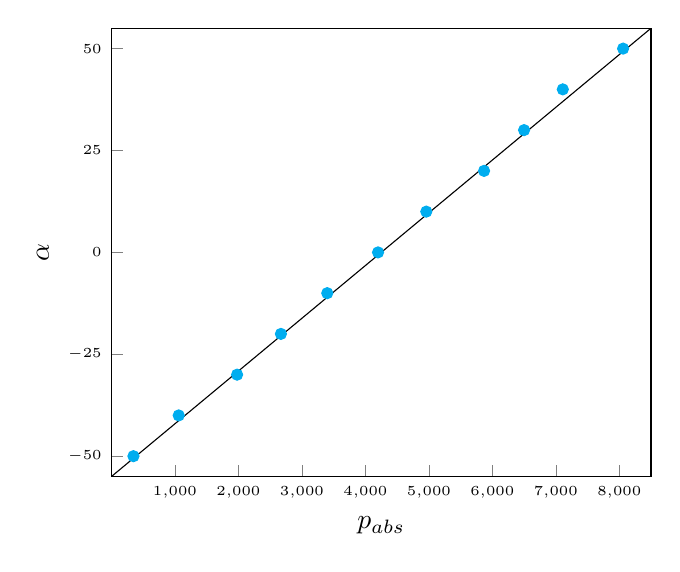
\begin{tikzpicture}
      \begin{axis}[
        xlabel={$p_{abs}$},
        ylabel={$\alpha$},
        xmin=0, xmax=8500,
        ymin=-55, ymax=55,
        xtick={1000,2000,3000,4000,5000,6000,7000,8000},
        ytick={-50,-25,0,25,50},
        xtick pos=left,
        ytick pos=left,
      ]

      \addplot[ no marks ] coordinates { (0,-55) (8500,55) };

      \addplot[ cyan, only marks ] coordinates {
        (347,-50) (1060,-40) (1980,-30) (2670,-20) (3400,-10) (4200,0) (4960,10) (5870,20) (6500,30) (7110,40) (8060,50)
      };

      \end{axis}
    \end{tikzpicture}
  \end{figure}
  
  The blue dots represent the measure values. We can clearly see some imprecision, which is due to the imperfection of the motor-mount and the string itself. Furthermore, the it's worth mentioning that the paddle moves from approximately -55 degrees to 55.

\end{document}